\section{Hash Table}
\begin{figure}[H]
        \centerline{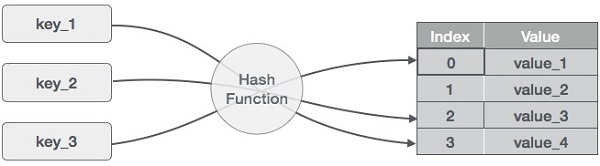
\includegraphics[scale=0.5]{figures/hash-tables/hash-function}}
        \caption{Hash Tables}
\end{figure}
Tabel hash adalah jenis struktur data di mana alamat atau nilai indeks elemen data dihasilkan dari fungsi hash. Itu membuat mengakses data lebih cepat karena nilai indeks berperilaku sebagai kunci untuk nilai data. Dengan kata lain tabel Hash menyimpan pasangan nilai kunci tetapi kuncinya dihasilkan melalui fungsi hashing. Jadi fungsi pencarian dan penyisipan elemen data menjadi lebih cepat karena nilai kunci itu sendiri menjadi indeks larik yang menyimpan data. Dalam Python, tipe data Kamus mewakili implementasi tabel hash. Kunci dalam kamus memenuhi persyaratan berikut.

\begin{enumerate}
\item Kunci kamus adalah hashable yaitu dihasilkan oleh fungsi hashing yang menghasilkan hasil unik untuk setiap nilai unik yang diberikan ke fungsi hash.
\item Urutan elemen data dalam kamus tidak tetap.
\end{enumerate}

Jadi kita melihat implementasi tabel hash dengan menggunakan tipe data kamus seperti di bawah ini.

\subsection{Mengakses Nilai dari Dictionary}
Untuk mengakses elemen kamus, Anda dapat menggunakan tanda kurung siku bersama dengan kunci untuk mendapatkan nilainya.
\begin{lstlisting}[language=Python, caption=Implementasi Hash Table]
# Declare a dictionary 
dict = {'Name': 'Angga', 'Age': 21, 'Class': 'Four'}

# Accessing the dictionary with its key
print("dict['Name']: ", dict['Name')]
print("dict['Age']: ", dict['Age'])
\end{lstlisting}

Ketika kode di atas dijalankan, menghasilkan hasil sebagai berikut:
\begin{lstlisting}[caption= Hasil Implementasi Hash Table]
dict['Name']:  Angga
dict['Age']:  21
\end{lstlisting}


\subsection{Update Dictionary}
Anda dapat memperbarui kamus dengan menambahkan entri baru atau pasangan nilai kunci, memodifikasi entri yang ada, atau menghapus entri yang ada seperti yang ditunjukkan di bawah ini dalam contoh sederhana.
\begin{lstlisting}[language=Python, caption=Implementasi Update Hash Table]
# Declare a dictionary
dict = {'Name': 'Angga', 'Age': 21, 'Class': 'Four'}
dict['Age'] = 20 # update existing entry
dict['College'] = "Poltekpos" # Add new entry
print("dict['Age']: ", dict['Age'])
print("dict['College']: ", dict['College'])
\end{lstlisting}

Ketika kode di atas dijalankan, menghasilkan hasil sebagai berikut:
\begin{lstlisting}[caption= Hasil Implementasi Update Hash Table]
dict['Age']:  20
dict['School']:  Poltekpos
\end{lstlisting}

\subsection{Delete Dictionary}
Anda dapat menghapus elemen kamus satu per satu atau menghapus seluruh konten kamus. Anda juga dapat menghapus seluruh kamus dalam satu operasi. Untuk menghapus seluruh kamus secara eksplisit, cukup gunakan pernyataan \textbf{del}.
\begin{lstlisting}[language=Python, caption=Implementasi Delete Hash Table]
# Declare a dictionary
dict = {'Name': 'Angga', 'Age': 21, 'Class': 'Four'}
del dict['Name'] # remove entry with key 'Name'
dict.clear()        # remove all entries in dict
del dict              # delete entire dictionary

print("dict['Age']: ", dict['Age'])
print("dict['School']: ", dict['School'])
\end{lstlisting}

Ini menghasilkan hasil berikut. Perhatikan bahwa pengecualian dimunculkan karena kamus setelah del dict tidak ada lagi.
\begin{lstlisting}[caption= Hasil Implementasi Delete Hash Table]
dict['Age']:
Traceback (most recent call last):
   File "test.py", line 8, in <module>
      print "dict['Age']: ", dict['Age'];
TypeError: 'type' object is unsubscriptable
\end{lstlisting}